\section{SCHEDULE AND EXPECTED RESULTS}

    In order to proceed with the work, it will be necessary to complete some independent steps, which will bring more solidity and make it easier to identify the problems and qualities of the work.
    
    \subsection{Capture Real Scenario Images}
        There is a need to deploy the solution on a real SoC or hardware platform to benchmark a real quadcopter application, or other fixed frame carrying controller such as those based on Pixhawk.
        In this way, it will be possible to recognize the possible impacts of angle deviations shown in images associated with roll and yaw poses on non normal angles to the water surface.
        
        Something to consider is the disturbance of the water surface with the airflow from the propellers of a real drone, with a promising ability to increase the discrepancy between images from different heights, also increasing the ability of the network to infer the different frames. 
        This behavior is expected because the surface disturbance will increase as the air flow demanded to move or hover. 
        Another variant is the sum of mass of inherent mass plus the payload, resulting in bigger inertia, and maybe bringing more challenges to the inference.
        Before any experiment with real drones, the platform should follow the frame design according to \ref{fig:buoy}, or equivalent, with buoy foots to avoid sinking or submerging essential electronic parts. The obstructions issues on camera is unknown. 
        
        
            \begin{figure}[!h]
                \centering
                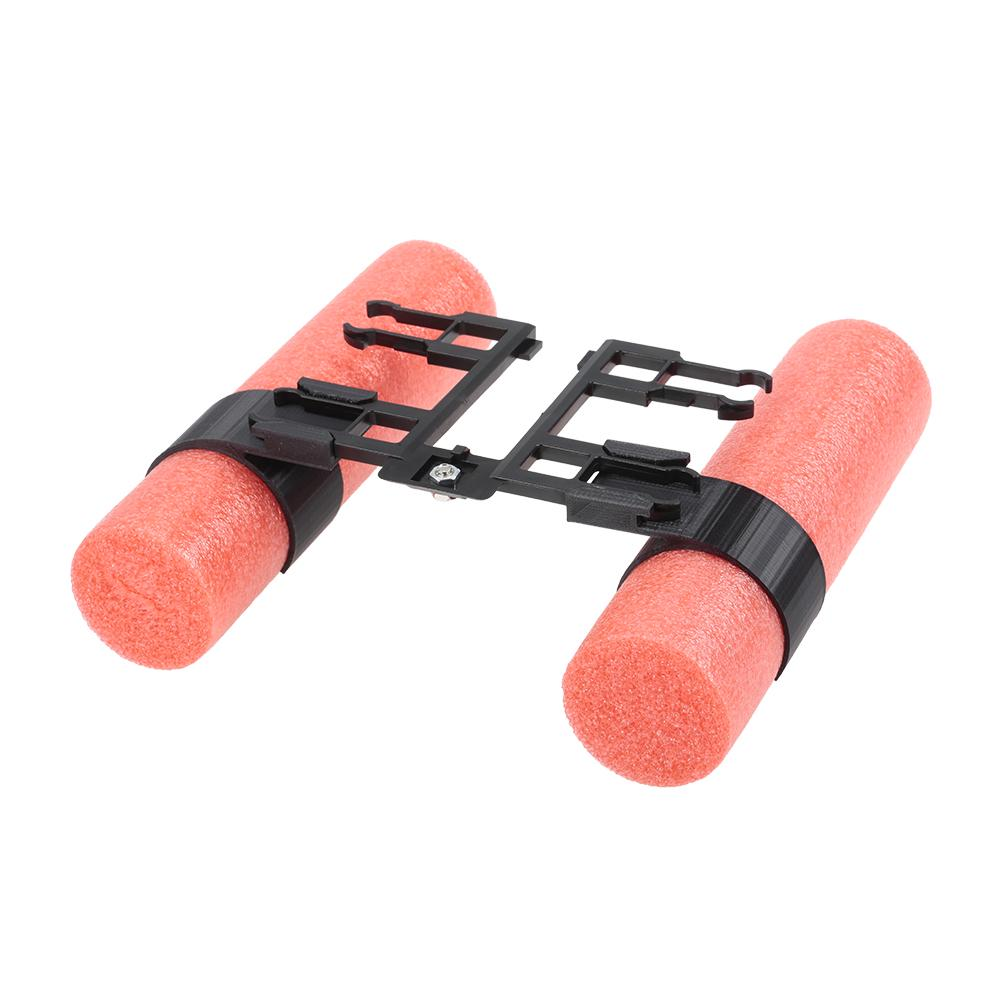
\includegraphics[width=13cm]{Images/buoy.jpeg}
                \caption{Example of quadcopter frame with buoy standings}
                \label{fig:buoy}
            \end{figure}
    
        A future test with rolling shutter cameras should be conducted to verify the impact of these distortions. This concern is due to high availability of these equipment in budget quadcopters, both embedded or aftermarket, like the options for entry level drones \cite{RollingShutter}.
    
    \subsection{Test on Different Architectures}
        Even with the promising results presented, the simplistic CNN architecture may be a bottleneck to unleash the real potential for the results, performance and hardware resource wise. 
        In the first field, we are aiming to the more powerful architectures, like the ones found in larger UAVs and for benchmarking purposes. 
        But the second field is related to the demand on low power devices, with MAV devices that can be benefited with smaller models, like MobileNet and alternatives. 

    
    \subsection{Submission to a journal event}
        Publication in journal is one of the goals with the preliminary material, with the writing process going along with the experiments, trials with new models and new data collections.
        The material should bring new insights in areas related to sensor fusion filters, aiming publications in events related to robotics, sensors and digital image processing.
    
    \begin{table}[htbp]
    \caption{Time execution schedule}
        \begin{center}
            \begin{tabular}{|c|c|c|c|}
            \hline
            \textbf{Task} & \textbf{Oct} & \textbf{Nov} & \textbf{Dec} \\
            \hline
            Test on Different CNN Architectures & X &  & \\
            \hline
            Submission on periodic event & & X &\\
            \hline
            Thesis Writing & X & X & \\
            \hline
            Defense & & & X \\
            \hline
            \end{tabular}
        \label{tabela_sumario}
        \end{center}
    \end{table}